\section*{Sources of bias in the SQF data}
\begin{figure}
    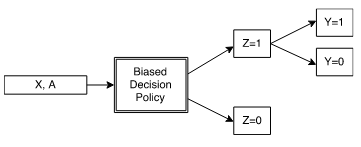
\includegraphics[width=0.7\textwidth]{../figures/selection_bias.png}
    \caption{Selection bias in the SQF data.}
    \label{fig:selection_bias}
\end{figure}
The major concern that has been identified in the literature for SQF data is how the data is generated in the first place. In their paper "Residual Unfairness" \cite{kallus} conceptualise the problem as shown in \autoref{fig:selection_bias}.
We define a person by their sensitive feature (A) and non-sensitive features (X). For each person in the population of interest a police officer decides whether to stop them or not. Based on this biased decision policy people are included in the sample (Z = 1) or they are not (Z = 0). But naturally we only observe further information on the people that were stopped. Only for them we can know the outcome of a stop, which constitutes the target of a classificaiton task.
\cite{kallus} distinguish between target population and training population in such scenarios. The target population is the one on which we want to use the ADM on while the training population are the observations the biased decision policy chose to include in the sample and on which the algorithm is trained.
In the SQF data we can see this form of bias by comparing the race distribution of NYC to the race distribution in the SQF data. From \autoref{fig:race_distributions} it is clear that in terms of race the SQF data does not represent the general population of the city. We can see that white people form the majority of the population in NYC, but only make up a tiny fraction of SQF stops. Black people in contrast are the third-largest ethnic group in NYC while they exceed any other group in the SQF data by far.
\autoref{fig:race_distributions} shows that selection bias might be at play in the decision of stopping a suspect.
\begin{figure}
    \centering
    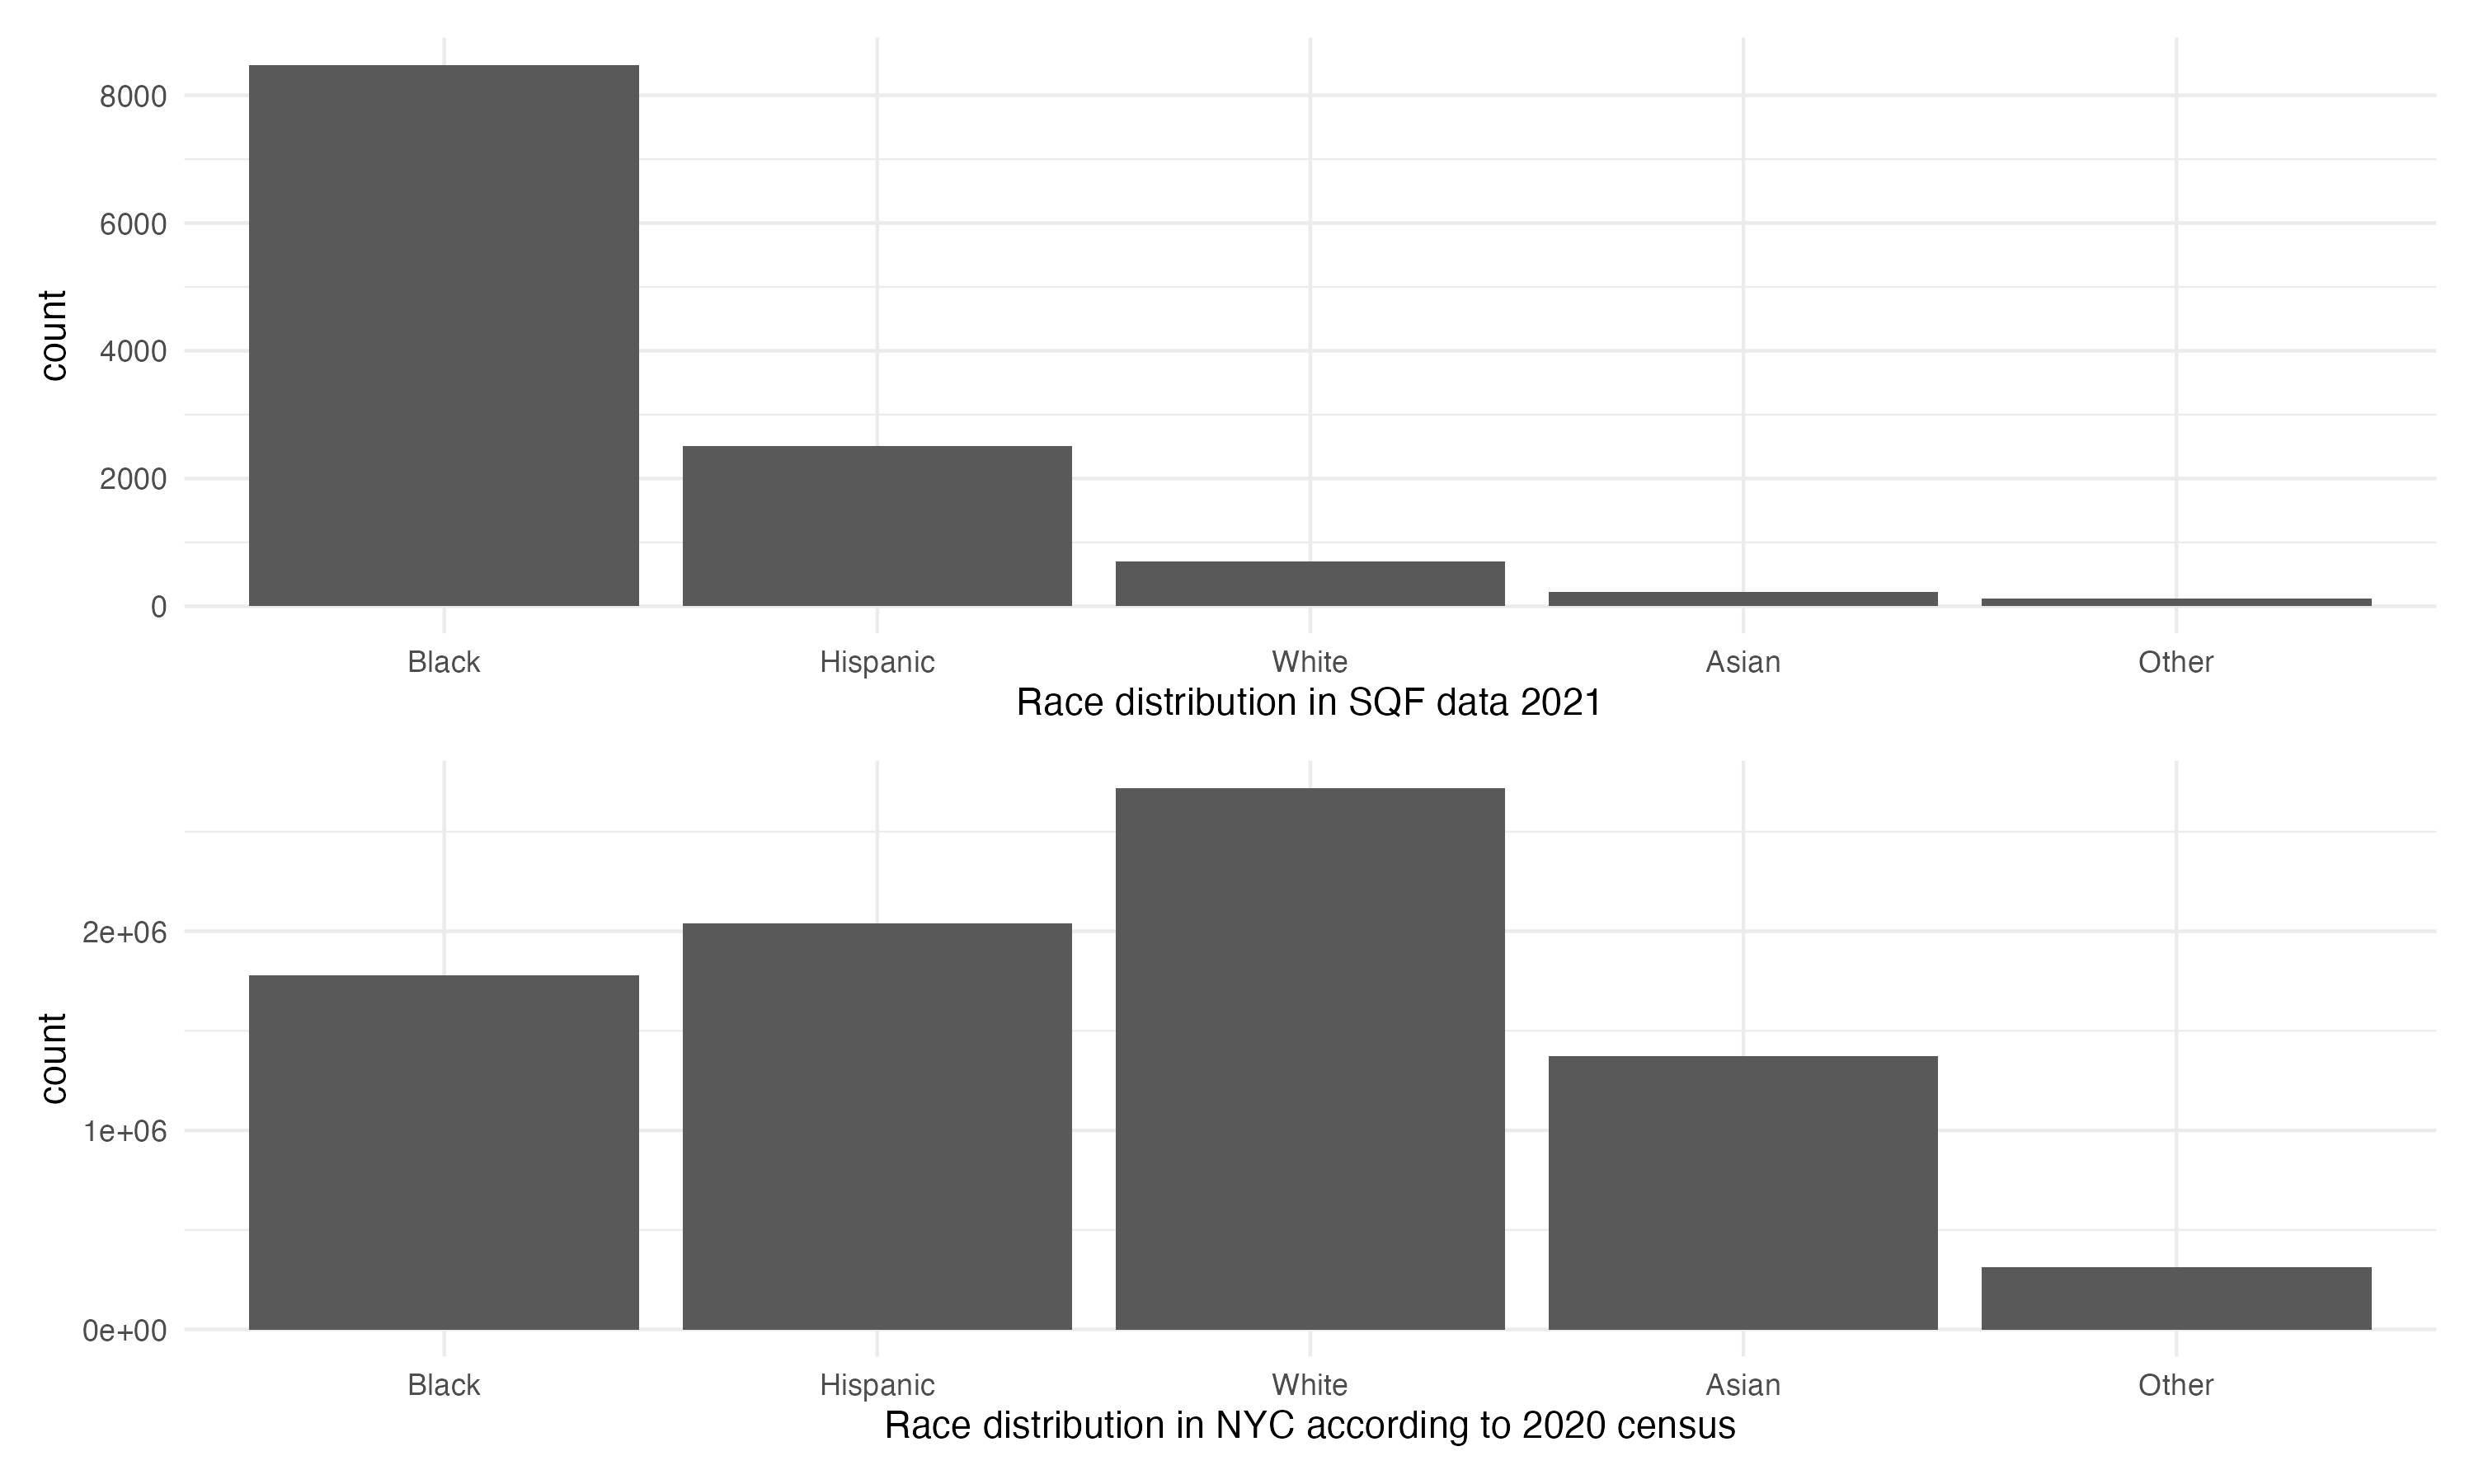
\includegraphics[width=0.7\textwidth]{../figures/sqf_case_study_plot6.png}
    \caption{Comparison of race distribution in the training and target population.}
    \label{fig:race_distributions}
\end{figure}

To get a more nuanced picture we also plot the true arrestment rate per ethnic group in the SQF 2023 data and find that White and Asian people have the highest arrestment rates and black people the lowest. This supports the argument that black people are stopped more leniently and there is a biased decision policy in place. The question is now how such biases can be addressed in fairness practice and why the group metrics did not detect any unfairness in our algorithm.
% The main message of this paper is that it is not that easy to adjust for fairness, when the data the algorithm learns from is biased. Ensuring Equal Opportunity or Equalized Odds on the training data does not generalize to the target population. The paper proposes a way to estimate the TRP and FPR in the target population. This is useful, when the fairness methods depends on the FPR and/or TPR. 
Why the group metrics did not show any unfairness in the algorithm can be answered ins a straight forward way. Group metrics offer a rather isolated view on fairness. They assess disparities in algorithimic predictions between protected groups rather than measuring the fairness of a whole situation. Thus, group metrics are not designed to detect selection bias. They work with the joint distribution of $Y, A, X, \hat{Y}$ and do not take any additional information into account. When we rely on the true label $Y$ (Separation) to detect unfairness but the true label itself is not reliabel (generated via an objective truth), then the group metrics cannot show this \cite{castelnovo2022}.

\section{Residual Unfairness}
The main methological goal of fairness methods designed to address biased samples is to prevent the problem of "bias in, bias out".
\cite{kallus} defines fairness via equal opportunity or equalised odds. They argue that even after fairness adjustments on the training population, such as thresholding, discrimination in the target population will remain.
Thus they design a way to estimate the true positive rate and false positive rate of the target population based on training data. A method that uses the TPR and FPR of the data (such as the method proposed by \cite{hardt2016}) can use these adjusted estimations instead and like this ensure fairness on the target population.


Residual Unfairness \cite{kallus} concepts defined in the paper:
Disparate benefit of the doubt: one group gets an advantage over the other by historically repeated better treatment of the group
Equal opportunity and Equalised odds --> from this they define "Inequity of Opportunity" to quantify fairness
First-order stochastic dominance (Def. 3): one group has consistently higher probability scores than the other
Strong disparate benefit of the doubt; Strong disparate benefit of the doubt,  strict;
Weak disparate benefit of the doubt, strict; Weak disparate benefit of the doubt on disparately endowed groups

Currently I understand it as follows:
The different disparate benfits of the doubt fromalise different historical treatment of groups.
We distinguish two groups in our population, a (advantaged) and b (disadvantaged). Within each group a and b we further dinstiguish between training population (Z=1) and target population (T=1).
My current understanding for Preposition 2: Some propositions now illustrate the scenario, in which repreated deiscriminatory treatment looks like this: For group a the scores in the training population are strictly lower than the scores in the target population. For group b the scores in the training population are strictly higher than in the atrget population. The consequence is that the classifier learn on average low scores for group a, resulting in lenient treatment of group a (which is beneficial in this scenario, $\hat{Y} = 1$ is desired). For group b the opposite mechanism occures, resulting in stricter treatment of group b.
My current understanding for proposition 3: When we design a classifier that that satisfies equal opportunity as fairness criterion under the situation described by preposition 2, then the classifier will not satisfy their definition of fainress/ will show Inequity of opportunity

Preposition 2:
For group a the scores of the target population are always strictly higher than
of the training population. This means that we will learn a comparatevily low threshold for group a.
When we employ the algorithm in the target population, group a member will receive the positive outcome
 more easily (receive benefit of the doubt) because the thresholds is so low. For group b
 the opposite is true. The scores in the training data are really high compared to the overall population.
 This means we learn a high threshold for group b. When the system is applied on the whole population it will
 be harder for a random person from group b to receive the advantage because their threshold is so high.
Applied on the SQF data this could translate as follows. First of all, the interpretation shifts. $\hat{Y} = 1$ is 
no longer desirable and we can interpret scores as riskscores $G_g^{E}$. This means a high thresholds for being classified as $\hat{Y} = 1$ is desirable, a low
threshold is undesirable. We assume that officers were more lenient to stop black individuals, which means that the scores (probability of actually having committed crime) in the training population
of black people are lower than the scores of the target population of black people.
$G_b^{Z=1} \preceq G_b^{T=1}$. This means we will learn a lower threshold for black people(???) \footnote{Why do we learn a lower threshold for black people. Maybe something like this happens: So when a group is super leniently stopped we will have many truly innocent and few truly guilty.}
When we apply the algorithm to the target population we will be more likely to classify black people as $\hat{Y} = 1$ because the threshold is so low. White people, on the other hand,
were selected more strictly. This means that the scores of white people in the training population are higher than the scores of white people in the target population.
$G_w^{Z=1} \succeq G_w^{T=1}$. This means we will learn a high threshold for white people. When we apply the algorithm to the target population we will be less likely to classify white
people as $\hat{Y} = 1$ because the threshold is so high. -- Still unsure if this makes sense, if a transfered it correctly.

For the other group we have many truly guilty and less truly innocent. When now 80\% of truly guilty are classified as guilty in the advantaged group then we would want want 80\% of
the truly guilty to be correctly labelled as guilty in the disadvantaged group. This would only results in lowering the threshold for the disadvantaged group
(so making it easier to predict them as guilty) if we predicted low risk scores for truly guilty people in the disadvantaged group
 Because for equal opportunity we are only looking at the people who were really guilty. So we are basically saying that the large proportion of truly
 innocent people in our sample of the disadvantaged leads to lower risk scores even in the truly guilty group of the disadvantaged (like a spill over effect).
 Only then it would make sense to say that a fairness intervention would compensate by setting lower thresholds for the disadvantaged group. Is this happening? 

Chapter 6: Case study on SQF data
Their main message is always, bias in, bias out. fairness interventions, done on the training data are not enough, if your sample is biased, your model will be biased (even after fairness interventions).
They show this in the following way. The goal is to predict innocence of an individual. Such an ADM could help officers
decide who to stop in the first place. The SQF data serves as training data and is naturally censored. The censoring process is that we only
observe innocence of a person if they were stopped. But the decision to stop someone could be based on a biased decision policy.
So we have our censored training data (SQF data). We know that this training data is not representative of the population of NYC in general defined via
location specific variables. Kallus and Zhou use train a logistic regression classifier on the SQF data as is and use post-processing proposed
by Hardt et al. to ensure Equal Opportunity or Equalized Odds. They use their a weighing technique (proposed by them and inspired by propensity score matching)
to simulate the target population. The fairness intervention in the training population produces group-specific thresholds that are then applied to the target population.
They use these fairness-adjusted threshold for the target population and still observe unfairness.

But of course they observe unfairness because the fairness intervention they do is a post-processing step and doesn't modifiy the classifier. What am i not getting here?